\documentclass[a4paper,12pt]{article}
\usepackage[a4paper,top=1.3cm,bottom=2cm,left=1.5cm,right=1.5cm,marginparwidth=0.75cm]{geometry}
\usepackage{cmap}
\usepackage{mathtext}
\usepackage[T2A]{fontenc}
\usepackage[utf8]{inputenc}
\usepackage[english,russian]{babel}
\usepackage{siunitx}
\usepackage{enumitem}
\usepackage{placeins}

\usepackage{graphicx}

\usepackage{wrapfig}
\usepackage{tabularx}
\usepackage{multirow}

\usepackage{hyperref}
\usepackage[rgb]{xcolor}
\hypersetup{
colorlinks=true,urlcolor=blue
}
\usepackage{amsmath,amsfonts,amssymb,amsthm,mathtools}
\usepackage{icomma}
\mathtoolsset{showonlyrefs=false}
\usepackage{euscript}
\usepackage{mathrsfs}
\DeclareMathOperator{\sgn}{\mathop{sgn}}
\newcommand*{\hm}[1]{#1\nobreak\discretionary{}
{\hbox{$\mathsurround=0pt #1$}}{}}

%%% Заголовок
\author{Макаров Лев Евгеньевич}
\title{Лабораторная работа №3.4.4

Петля гистерезиса (статический метод)
}
\date{\today}


\begin{document}

\begin{titlepage}
	\begin{center}
		{\large МОСКОВСКИЙ ФИЗИКО-ТЕХНИЧЕСКИЙ ИНСТИТУТ (НАЦИОНАЛЬНЫЙ ИССЛЕДОВАТЕЛЬСКИЙ УНИВЕРСИТЕТ)}
	\end{center}
	\begin{center}
		{\large Физтех-школа фотоники, электроники и молекулярной физики}
	\end{center}
	
	
	\vspace{4.5cm}
	{\huge
		\begin{center}
			{\bf Отчёт о выполнении лабораторной работы 3.4.4}\\
			Петля гистерезиса (статический метод)
		\end{center}
	}
	\vspace{2cm}
	\begin{flushright}
		{\LARGE Автор:\\ Макаров Лев Евгеньевич \\
			\vspace{0.2cm}
			Б04-306}
	\end{flushright}
	\vspace{8cm}
	\begin{center}
		Долгопрудный 2024
	\end{center}
\end{titlepage}

\section{Введение}

\textbf{Цель работы:} 
\begin{enumerate}
	\item наблюдение начальной кривой намагничивания ферромагнетиков и предельной петли гистерезиса
\end{enumerate}

\textbf{В работе используются:} 
\begin{itemize}
    \item источник питания
    \item тороид
    \item соленоид
    \item баллистический гальванометр с осветителем и шкалой
    \item амперметр
    \item вольтметр
    \item магазин сопротивлений
    \item лабораторный автотрансформатор (ЛАТР)
    \item разделительный трансформатор
    \item понижающий трансформатор
    \item интегрирующая цепочка
    \item электронный осциллограф
    \item делитель напряжения
\end{itemize}
\medskip

\section{Теоретические сведения}

К ферромагнетикам принадлежат железо, никель, кобальт, гадолиний, их многочисленные сплавы с другими металлами. К ним примыкают ферриты -- диэлектрики со структурой антиферромагнетика.

Ферромагнетики -- вещества, которые при определенной температуре обладают самопроизвольной намагниченностью $\boldsymbol{M}$ в отсутствие внешнего магнитного поля. В ферромагнетиках образуются отдельные намагниченные области – домены (от $10^{-2}$ до $10^{-6}$ см$^3$), магнитные моменты в которых ориентируются параллельно.

Зависимость вектора магнитной индукции $\boldsymbol{B}$ ферромагнетика от вектора напряженности магнитного поля $\boldsymbol{H}$ нелинейна. В системе СИ эта связь имеет вид
\begin{equation} \label{eq:BM}
    \boldsymbol{B} = \mu_0(\boldsymbol{H} + \boldsymbol{M})
\end{equation}

При циклическом перемагничивании зависимость (\ref{eq:BM}) изображается замкнутой кривой - симметричной петлей гистерезиса (рис. \ref{ris:hysteresis}), где $\pm \boldsymbol{H}_c$ – значение напряженности магнитного поля, необходимое для полного размагничивания ферромагнетика (коэрцитивная сила); $\pm \boldsymbol{B}_r$ – магнитная индукция, которую имеет ферромагнетик при напряженности внешнего магнитного поля, равную нулю (остаточная намагниченность); $\pm \boldsymbol{B}_s$ – значение магнитной индукции, при которой материал достигает насыщения (намагниченность насыщения)\footnote{Кривая, изображающая зависимость $B(H)$, практически совпадает с зависимостью $M(H)$, поскольку второй член в выражении (\ref{eq:BM}), в малых полях, существенно превосходит первый}.
\begin{figure}[!h]
    \center{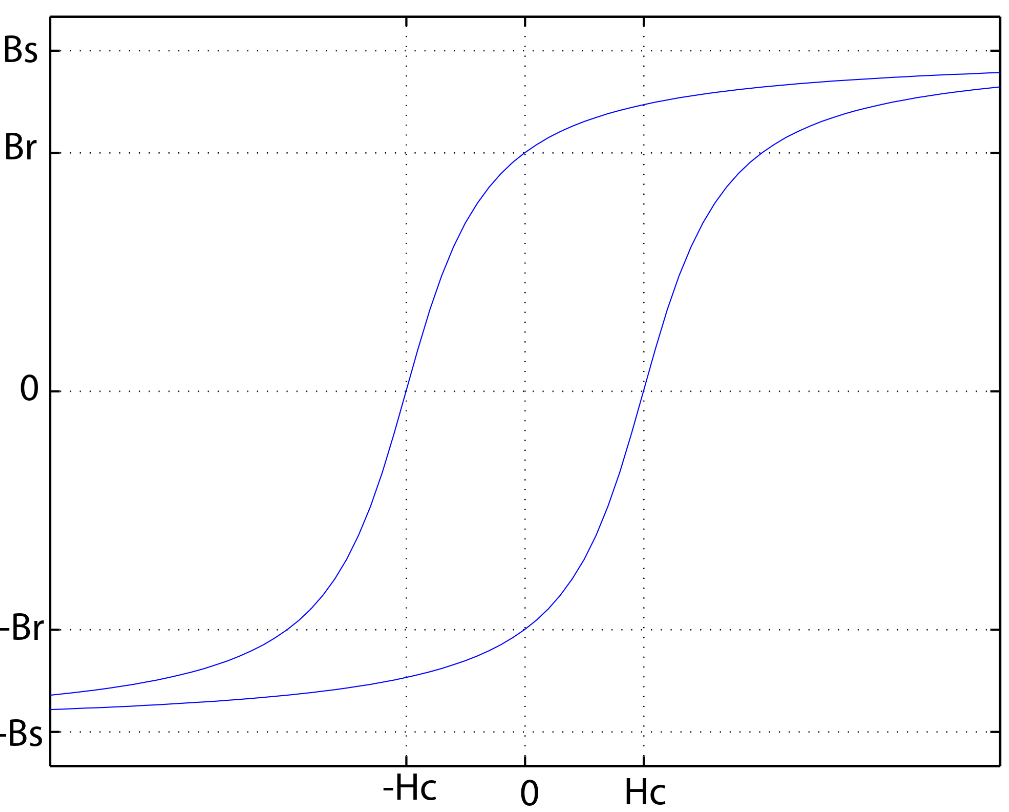
\includegraphics[width=10cm]{hist.png}}
    \caption{Петля гистерезиса ферромагнетика.}
    \label{ris:hysteresis}
\end{figure}

\section{Экспериментальная установка}

\subsection{Статический метод}

\begin{figure}[h]
    \centering
    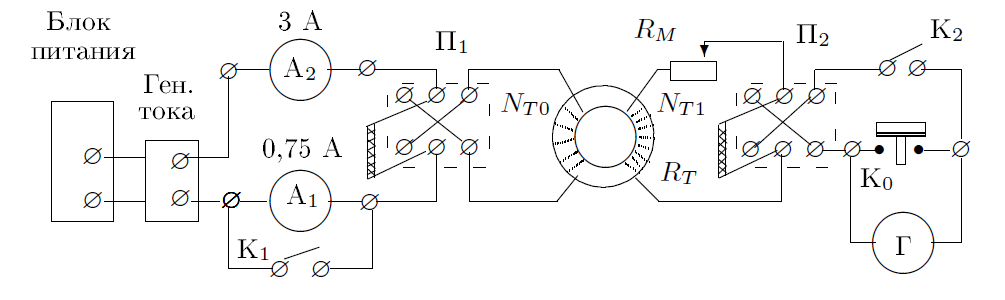
\includegraphics[width=10cm]{ust-1.png}
    \caption{Схема установки для исследования петли гистерезиса}
    \label{pic:gist}
\end{figure}

\begin{figure}[h]
    \centering
    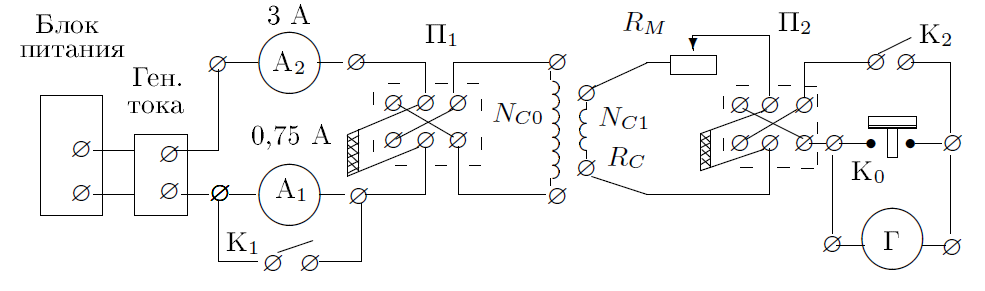
\includegraphics[width=10cm]{ust-2.png}
    \caption{Схема установки для калибровки гальванометра}
    \label{pic:galv}
\end{figure}

После снятия петли гистерезиса необходимо размагнитить сердечник, подключив его к цепи переменного тока, постепенно снижая его амплитуду. Только затем следует приступать к снятию основной кривой намагничивания.

\subsection{Динамический метод}

Схема экспериментальной установки показана на рис. 3.

Действующее значение переменного тока в обмотке N0 измеряется амперметром А (мультиметром GDM). Последовательно с амперметром включено сопротивление $R_{0}$, напряжение с которого подается на вход X электронного осциллографа (ЭО). Это напряжение пропорционально току в обмотке $N_{0}$, а следовательно и напряженности H магнитного поля в образце.

Для измерения магнитной индукции B с измерительной обмотки $N_\text{И}$ на вход интегрирующей RC -цепочки подается напряжение $U_\text{И}$ (UВХ), пропорциональное производной $\dot{B}$, а с выхода снимается напряжение $U_{C}$($U_\text{ВЫХ}$), пропорциональное величине B , и подается на вход Y осциллографа.
Замкнутая кривая, возникающая на экране, воспроизводит в некотором масштабе (различном для осей X и Y ) петлю гистерезиса. Чтобы придать этой кривой количественный смысл, необходимо установить масштабы изображения, т.е. провести калибровку каналов X и Y ЭО. Для этого, во-первых, надо узнать, каким напряжениям (или токам) соответствуют амплитуды сигналов, видимых на экране, и во-вторых,  каким значениям B и H соответствуют эти напряжения
(или токи).

\begin{figure}[h!]
    \centering
    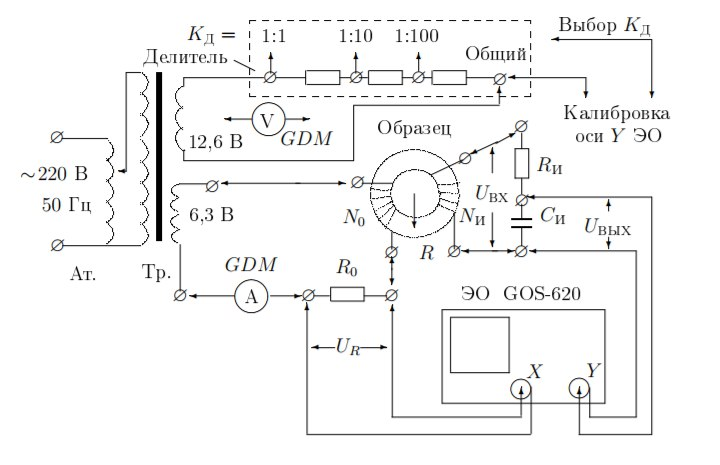
\includegraphics[width=\linewidth]{ust-3.jpg}
    \caption{Схема установки для исследования намагничивания образцов}
    \label{pic:caliber}
\end{figure}

\begin{itemize}
    \item
        Напряженность магнитного поля $H$ в тороиде зависит от тока, текущего в намагничивающей обмотке:
        \begin{equation}\label{eq:H}
            H = \frac{N_{T_0}}{\pi D} I;
        \end{equation}
    \item
        Связь между отклонением зайчика баллистического гальванометра в делениях $\Delta x$ и изменением магнитной индукции $\Delta B$ в сердечнике тороида:
        \begin{equation}\label{eq:B}
            \Delta B = \mu_0 \left(\frac{d_C}{d_T}\right)^2 \frac{N_{C_0}}{N_{T_1}} \frac{N_{C_1}}{l_C} \Delta I_1 \frac{\Delta x}{\Delta x_1}.
        \end{equation}
\end{itemize}

\section{Результаты измерений и обработка данных}

\subsection{Подготовка к работе}

\begin{enumerate}
    \item Соберем схему согласно рис. \ref{pic:gist}. Расположим ключи так, чтобы было удобно снимать расчеты.
    \item Включим генератор и амперметр в сеть, установим необходимый режим работы. Проверим, как меняется ток в первичной обмотке. Вернемся к нулевому току.
    \item Установим сопротивление магазина $R_M = 100$ Ом. Включим осветитель гальванометра.
    \item Установим максимальный ток $I_{max} = 1,46$ А. Замкнем ключ К1. Следя за каждым отклонением зайчика, пройдем всю кривую намагничивания, чтобы убедиться, что он нигде не выходит за пределы шкалы.
\end{enumerate}

\subsection{Предельная петля гистерезиса}

\begin{enumerate}[resume]
    \item Пройдем по половине петли гистерезиса и замерим все положения тока и отклонения зайчика. Сумма отклонений зайчика по различным участкам цепи одинаков в пределах 10\%. Результаты измерений в таблице \ref{table:1}
\end{enumerate}


\FloatBarrier
\begin{table}[]
    \centering
    \caption{\textit{Начальная кривая намагничивания}}
    \begin{tabular}{|l|l|l|l|l|l|}
        \hline
        Положение & I, mA   & $\Delta x$, мм & H, А/м & $\Delta B$, Т              & B, Т  \\ \hline
        0        & 0.0 & 1.7    & 0.0    & 0.028 & 0     \\ \hline
        1        & 15.35  & 3.2    & 85.5   & 0.055 & 0.028 \\ \hline
        2        & 28.11  & 3.5    & 156.6  & 0.060 & 0.083 \\ \hline
        3        & 39.17  & 0.9    & 218.2  & 0.015 & 0.143 \\ \hline
        4        & 44.52  & 2.8    & 248.0  & 0.048 & 0.158 \\ \hline
        5        & 56.03   & 2.1    & 312.1  & 0.036 & 0.206 \\ \hline
        6        & 66.72   & 2.9    & 371.7  & 0.050 & 0.242 \\ \hline
        7        & 94.99   & 3.1    & 529.1  & 0.052 & 0.292 \\ \hline
        8        & 157.35  & 4.0    & 876.5  & 0.068 & 0.345 \\ \hline
        9        & 250.56  & 6.7    & 1395.7 & 0.113  & 0.412 \\ \hline
        10       & 514.50   & 13.2   & 2866.0 & 0.225  & 0.526 \\ \hline
        11       & 1460.00    & 12.0   & 8132.8 & 0.205  & 0.750 \\ \hline
    \end{tabular}
\end{table}
\FloatBarrier

\FloatBarrier

\begin{table}[!h]
    \centering
    \caption{\textit{Прохождение цикла гистерезиса}}
    \begin{tabular}{|l|l|l|l|l|l|l|l|l|l|l|l|}
        \cline{1-3} \cline{5-6} \cline{8-9} \cline{11-12}
        участок   & \multicolumn{1}{c|}{1} &         &  & \multicolumn{1}{c|}{2} &         &  & \multicolumn{1}{c|}{3} & \multicolumn{1}{c|}{} &  & \multicolumn{1}{c|}{4} &         \\ \cline{1-3} \cline{5-6} \cline{8-9} \cline{11-12} 
        положение & I, ma                  & Delta x &  & I, ma                  & Delta x &  & I, ma                  & Delta x               &  & I, ma                  & Delta x \\ \cline{1-3} \cline{5-6} \cline{8-9} \cline{11-12} 
        11        & 1460,00                &         &  & 1458,50                & 12,8    &  & 1459,50                &                       &  & 1458,50                & 12,7    \\ \cline{1-3} \cline{5-6} \cline{8-9} \cline{11-12} 
        10        & 514,50                 & 12,4    &  & 514,20                 & 14,3    &  & 514,40                 & 12,0                  &  & 514,20                 & 14,1    \\ \cline{1-3} \cline{5-6} \cline{8-9} \cline{11-12} 
        9         & 250,56                 & 11,0    &  & 250,56                 & 11,3    &  & 250,61                 & 11,5                  &  & 250,56                 & 11,2    \\ \cline{1-3} \cline{5-6} \cline{8-9} \cline{11-12} 
        8         & 157,35                 & 7,6     &  & 157,28                 & 16,2    &  & 157,31                 & 7,1                   &  & 157,27                 & 16,1    \\ \cline{1-3} \cline{5-6} \cline{8-9} \cline{11-12} 
        7         & 94,99                  & 5,8     &  & 95,01                  & 16,0    &  & 95,10                  & 5,2                   &  & 94,96                  & 15,9    \\ \cline{1-3} \cline{5-6} \cline{8-9} \cline{11-12} 
        6         & 66,72                  & 2,6     &  & 66,72                  & 9,0     &  & 66,75                  & 2,6                   &  & 66,73                  & 9,0     \\ \cline{1-3} \cline{5-6} \cline{8-9} \cline{11-12} 
        5         & 56,03                  & 1,3     &  & 56,01                  & 17,6    &  & 56,03                  & 1,3                   &  & 56,02                  & 17,7    \\ \cline{1-3} \cline{5-6} \cline{8-9} \cline{11-12} 
        4         & 44,52                  & 1,3     &  & 44,51                  & 11,1    &  & 44,52                  & 1,4                   &  & 44,51                  & 11,1    \\ \cline{1-3} \cline{5-6} \cline{8-9} \cline{11-12} 
        3         & 39,17                  & 0,8     &  & 39,17                  & 16,3    &  & 39,17                  & 0,6                   &  & 39,17                  & 16,0    \\ \cline{1-3} \cline{5-6} \cline{8-9} \cline{11-12} 
        2         & 28,11                  & 1,4     &  & 28,11                  & 6,6     &  & 28,11                  & 1,2                   &  & 28,11                  & 6,4     \\ \cline{1-3} \cline{5-6} \cline{8-9} \cline{11-12} 
        1         & 15,35                  & 2,0     &  & 15,36                  & 5,3     &  & 15,36                  & 1,7                   &  & 15,36                  & 5,1     \\ \cline{1-3} \cline{5-6} \cline{8-9} \cline{11-12} 
        0         & 0,00                   & 3,5     &  & 0,00                   &         &  & 0,00                   & 3,3                   &  & 0,00                   &         \\ \cline{1-3} \cline{5-6} \cline{8-9} \cline{11-12} 
    \end{tabular}
    \label{table:1}
\end{table}

\FloatBarrier

\subsection{Калибровка гальванометра}

\begin{enumerate}[resume]
    \item Соберем схему на рис. \ref{pic:galv}.
    \item Уменьшим сопротивление на магазине на $R_C$ до $R'_M = 40$ Ом.
    \item Установим генератор на максимум тока. Замкнем ключ П1. Замерим отклонение при изменении от максимального тока до 0. $I_\text{max} = 1,46$ А, $\Delta x = 7,9$ см.
\end{enumerate}

\subsubsection{Начальная кривая намагничивания}

\begin{enumerate}[resume]
    \item Размагнитим образец.
    \item Подсоединим тороид к сети, Установим тумблер генератора на минимальный ток. Снимем начальную кривую намагничивания, скачками увеличивая ток до $I_\text{max}$.
    \item Запишем параметры установки: $d_T = 1$ см, $D = 10$ см. Отключим питание и разберем схему.
\end{enumerate}

\subsection{Обработка результатов}

Используя формулы (\ref{eq:H}) и (\ref{eq:B}) рассчитаем $H = f_1(I)$ и $\Delta B = f_2 (\Delta x)$ для начальной и предельной петель гистерезиса. По полученным данным (табл.\ref{table:limit}-\ref{table:start}) построим петлю гистерезиса $B = f (H)$. Стоит отметить, что для выполнения естественного условия $f(0) = 0$, к нашим результатам была прибавлена величина $B_0 = 1,38$ Тл. 

\begin{figure}[H]
    \center{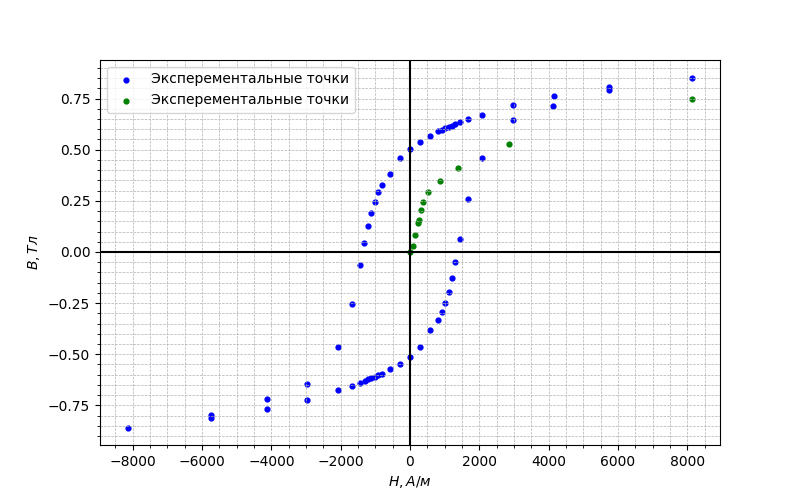
\includegraphics[scale=1]{graph-petlya.png}}
    \caption{Зависимость $B = f(I)$.}
    \label{ris:B=f(I)}
\end{figure}


По графику найдём коэрцитивную силу $H_c$, индукцию насыщения $B_s$ и остаточную индукцию $B_r$. Более того, можно вычислить максимальное значение дифференциальной магнитной проницаемости $\mu$ для начальной кривой намагничивания.

\begin{table}[H]
    \caption{Анализ петли гистерезиса.}
    \label{table:result}
    \begin{tabular}{|c|c|c|c|}
        \hline
        $H_C$, А/м   & $B_S$, Тл         & $B_r$, Тл    & $\mu_{диф}$  \\ \hline
        $1600\pm 11$ & $1,410 \pm 0,010$ & $0,810\pm 0,010$ & $470 \pm 20$ \\ \hline
    \end{tabular}
\end{table}




\end{document}